\documentclass{article}
\usepackage{graphicx}

\begin{document}

\title{Team Meeting 3 Summary}
\author{Christian Plourde 26572499\\*
		Ayush Kharade 40042388\\*
		Daniel Vellucci 27416288\\*
		Samer Yazbeck 40049573\\*
		Luciano Porchet 40048537
		}
\date{September 28th, 2019}

\maketitle

\newpage

\section{Meeting Duration}
90 Minutes

\section{Notes}

\subsection{Summary}
Meeting was centered around building the proposal document as a team. The main character model was completed. Name of game: Mistborn - Ragnarok

\subsection{Proposal Presentation}
The presentation will consist of 4 parts: Introduction, Story and Setting, Mechanics, and art direction.
\begin{description}
\item Introduction - Title and tagline (introduce) - Daniel
\item Story and Setting - Explain backstory and setting, explain traumatic events leading to main character becoming mistborn (losing his crew) - Chris
\item Mechanics - Explain platformer mechanics and spend more time on the metal / potion consuming parts. Explain enemies, and how to deal with them (only fight using pewter or sneaking past) - Platforming and puzzle mechanics explained by Daniel and Metals/powers and enemies explained by Luciano
\item Related Games - Trine, INSIDE, Hollow Knight, and Claw - Ayush
\item Art Direction - How the art references resembles our setting. Explain screenshot and box art. Need a lot of images, mistborn book image, screen shots, and art - Samer
\end{description}

\subsection{Enemies}
\begin{description}
\item Added Koloss Enemy (Large ogre like monster)
\end{description}

\subsection{UI Element}
\begin{description}
\item Health bar - numeric points or hearts
\item Icons for metals carried by player
\item Simple menu to start game
\end{description}

\subsection{How metals/solutions should look}
\begin{description}
\item Pewter looks like power stone (purple)
\item Iron (orange)
\item Steel (silver)
\item Pewter can have a negative side effect (keep losing health while it is active)
\end{description}

\subsection{Supporting Art}
  \begin{figure}[!htb]
  \caption {Basic character model layout}
    \center{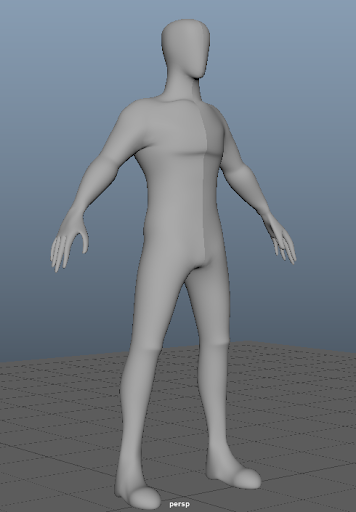
\includegraphics[width=5cm, height=5cm]
    {3D_model_body_basic.png}}
  \end{figure}

  \begin{figure}[!htb]
  \caption {Basic character with lighting}
    \center{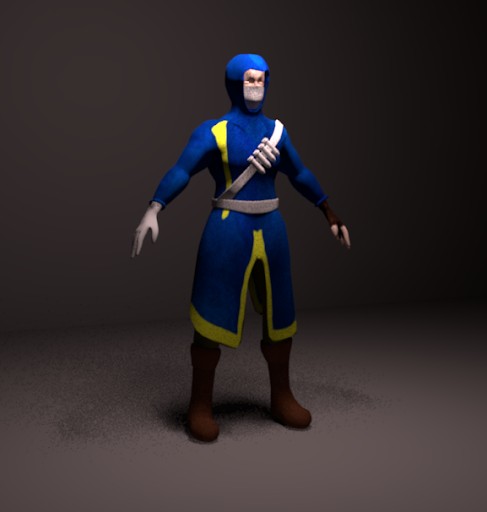
\includegraphics[width=5cm, height=5cm]
    {character_lit.png}}
  \end{figure}

  \begin{figure}[!htb]
  \caption {Basic character with lighting}
    \center{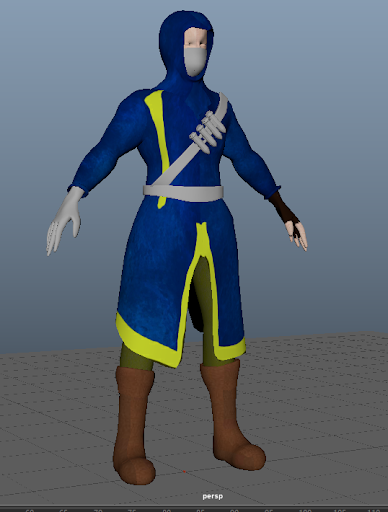
\includegraphics[width=5cm, height=5cm]
    {character_unlit.png}}
  \end{figure}

  \begin{figure}[!htb]
  \caption {Possible icon for iron solution}
    \center{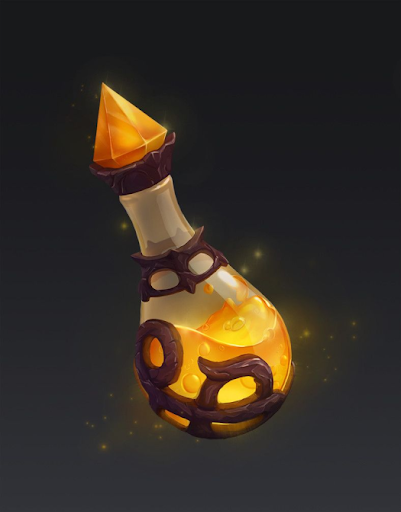
\includegraphics[width=5cm, height=5cm]
    {orange_vial.png}}
  \end{figure}

  \begin{figure}[!htb]
  \caption {Possible icon for steel solution}
    \center{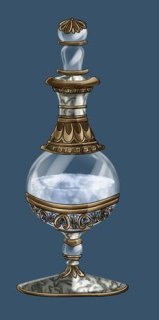
\includegraphics[width=5cm, height=5cm]
    {steel_solution.png}}
  \end{figure}

  \begin{figure}[!htb]
  \caption {Possible icon for pewter solution}
    \center{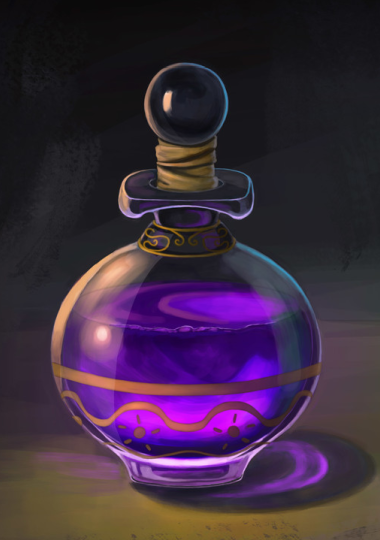
\includegraphics[width=5cm, height=5cm]
    {pewter_solution.png}}
  \end{figure}


\end{document}